% This must be in the first 5 lines to tell arXiv to use pdfLaTeX, which is strongly recommended.
\pdfoutput=1
% In particular, the hyperref package requires pdfLaTeX in order to break URLs across lines.

\documentclass[11pt]{article}

% Remove the "review" option to generate the final version.
\usepackage[review]{ACL}

% Standard package includes
\usepackage{times}
\usepackage{latexsym}



% For proper rendering and hyphenation of words containing Latin characters (including in bib files)
\usepackage[T1]{fontenc}
% For Vietnamese characters
% \usepackage[T5]{fontenc}
% See https://www.latex-project.org/help/documentation/encguide.pdf for other character sets

% This assumes your files are encoded as UTF8
\usepackage[utf8]{inputenc}

% This is not strictly necessary and may be commented out.
% However, it will improve the layout of the manuscript,
% and will typically save some space.
\usepackage{microtype}

% This is also not strictly necessary and may be commented out.
% However, it will improve the aesthetics of text in
% the typewriter font.

\usepackage{inconsolata}
\usepackage{amsmath}
\usepackage{graphicx}
\usepackage{comment}
\usepackage{amssymb}
\usepackage[inkscapeformat=png]{svg}
\usepackage{paralist}

% If the title and author information does not fit in the area allocated, uncomment the following
%
%\setlength\titlebox{<dim>}
%
% and set <dim> to something 5cm or larger.

% If the title and author information does not fit in the area allocated, uncomment the following
%
%\setlength\titlebox{<dim>}
%
% and set <dim> to something 5cm or larger.

\title{RIFF: Rephrasing Inputs for Few-shot Fine-tuning of Language Models}

% Author information can be set in various styles:
% For several authors from the same institution:
% \author{Author 1 \and ... \and Author n \\
%         Address line \\ ... \\ Address line}
% if the names do not fit well on one line use
%         Author 1 \\ {\bf Author 2} \\ ... \\ {\bf Author n} \\
% For authors from different institutions:
% \author{Author 1 \\ Address line \\  ... \\ Address line
%         \And  ... \And
%         Author n \\ Address line \\ ... \\ Address line}
% To start a seperate ``row'' of authors use \AND, as in
% \author{Author 1 \\ Address line \\  ... \\ Address line
%         \AND
%         Author 2 \\ Address line \\ ... \\ Address line \And
%         Author 3 \\ Address line \\ ... \\ Address line}

\author{Saeed Najafi \and
  Alona Fyshe \\
  Department of Computing Science, University of Alberta, Canada\\
  \texttt{\{snajafi,alona\}@ualberta.ca} \\}

\begin{document}
\maketitle
\begin{abstract}
Pre-trained Language Models (PLMs) have shown remarkable performance when fine-tuned for downstream text processing tasks. Recently, researchers have effectively guided PLMs to perform specific tasks by optimizing input prompts (prompt optimization) or adjusting a small number of model parameters (efficient tuning). In this study, we explore the impact of altering the input text of the original task while fine-tuning language models with these recent prompt optimization and efficient tuning methods. To most effectively rewrite the input text, we apply a learning objective based on Maximum-Marginal Likelihood estimation in a few-shot setting. Experimenting with seven few-shot text classification datasets, we show that enriching training examples with the input text's paraphrases at train and test time significantly enhances the performance of recent prompt optimization and efficient tuning techniques.
\end{abstract}


\section{Introduction}
Multiple Pre-trained Language Models (PLMs), such as BERT~\cite{devlin-etal-2019-bert}, RoBERTa~\cite{DBLP:journals/corr/abs-1907-11692}, T5~\cite{DBLP:journals/corr/abs-1910-10683}, and GPT2~\cite{radford2019language}, have demonstrated remarkable performance when fine-tuned for downstream text processing tasks. PLM variants with less than 1 billion parameters are easier to train end-to-end with commodity hardware. However, very recent PLMs have been trained with a few hundred billion parameters, including PaLM-2 (540B)\cite{anil2023palm}, GPT3 (175B)\cite{brown2020language}, OPT (175B)\cite{zhang2022opt}, or Llama-2 (70B)\cite{touvron2023llama}. Training all parameters of these models end-to-end is not straightforward unless done with a dedicated cluster of specialized hardware.

In response, NLP research have developed effective techniques to control or alter the behavior of PLMs by updating the input context through prompt optimization~\cite{DBLP:journals/corr/abs-2107-13586} or adapting a few additional parameters within the network itself~\cite{DBLP:journals/corr/abs-2106-09685}.
However, current PLM control techniques have not considered altering the \textit{original input text} to improve the performance of the model.  Here, we investigate this idea by training a secondary smaller PLM to paraphrase the original input at train and test time, thus augmenting the existing data and improving model performance.

Our inspiration comes from interactions with young children.
Determining what a child knows is challenging because they can be sensitive to the wording of the question~\cite{childBook}. Adults are also influenced  by different wordings of a question.  For example, opinion polling has been found to be sensitive to the wording of questions~\cite{Broughton1995}. Just like we rephrase questions for humans, we should consider rephrasing input text while querying a PLM. For instance, while classifying the topic of a sentence, phrases related to time may be irrelevant and could be removed to simplify the modeling problem. Slight changes to wording could result in the model producing a correct prediction.

We explore the integration of paraphrased input texts during both the training and testing phases. At \emph{training time}, augmenting data through paraphrase generation has been shown to enhance performance~\cite{wei-zou-2019-eda, feng-etal-2021-survey, DBLP:journals/corr/abs-2106-07499}. We broaden the scope of previous investigations by using paraphrase augmentation in tandem with recent prompt optimization and efficient tuning methods. At \emph{test time}, recent works have used ensemble predictions with various optimized prompts and tuned weights~\cite{izmailov2019averaging, allingham2023simple, li-etal-2023-making}. We further contribute to this line of work by incorporating ensemble predictions based on input paraphrases, again in concert with prompt optimization and efficient tuning techniques.

We start by pre-training a smaller language model on noisy paraphrases generated by a large language model (i.e., ChatGPT). Subsequently, we explore various training objectives for fine-tuning this paraphrase generator with feedback from the main task's language model.
\begin{comment}
Our extensive ablation experiments suggest that using Maximum-Marginal Likelihood (MML) gradient estimation with reward normalization applied to the language model's feedback is effective. Additionally, we propose a mixed decoding strategy for fine-tuning the paraphrase generator along with a Kullback-Leibler (KL) penalty applied between the pre-trained model and the current paraphrase model.
\end{comment}
Our experiments on seven text classification datasets demonstrate that incorporating paraphrase augmentation during both training and testing phases significantly enhances the performance of discrete/soft prompt optimization and efficient tuning techniques. In summary, our contributions are as follows:
\begin{itemize}
\item We propose an efficient idea for Rephrasing Inputs for Few-shot Fine-tuning of language models (RIFF) with prompt optimization and efficient tuning methods.
\item We conduct a comprehensive study on various learning objectives for fine-tuning a paraphrase generator using feedback from the main language model.
\item Our augmentation experiments on seven text classification datasets reveal that paraphrase generation, when combined with prompt optimization and adaptation techniques, is a simple yet effective approach for tuning language models on commodity hardware, closing the gap with fine-tuning all the parameters.
\end{itemize}

\section{Problem Formulation}
We focus on classification problems in Natural Language Understanding (NLU) tasks where we have access to a mini-batch of supervised training examples $B_{\text{supp}} = \{(x_i, y_i)\}_{i=1}^{N}$. Our goal is to update the parameter set $\theta_{\text{lm}}$ for a language model by maximizing the probability of the class label $y_i$ given the input $x_i$: $P_{\theta_{\text{lm}}} (y_i | x_i)$.

Here, we augment $B_{\text{supp}}$ with semi-supervised examples. In particular, we generate $M$ paraphrases for each $x_i$ using the paraphrase generator $P_{\theta_{\text{par}}} (z_{i,j} | x_i)$, where $z_{i,j}$ represents the $j$-th paraphrase for the input $x_i$.  In the optimal case, this paraphrase will preserve semantic meaning but vary syntactic/lexical form.

We then incorporate the generated paraphrases to create a new mini-batch of examples $B_{\text{s+p}} = B_{\text{supp}} \cup B_{\text{para}}$.  Using this augmented mini-batch, we then optimize the following objective function:
\begin{multline}
J_{\theta_{\text{lm}}} := \sum_{i=1}^N \{\log P_{\theta_{\text{lm}}} (y_i | x_i) + \\
\frac{1}{M} \sum_{j=1}^{M} \log P_{\theta_{\text{lm}}} (y_i | z_{i,j})\}
\label{lmfp-augmentation-objective}
\end{multline}

\subsection{Baseline LM Tuning Techniques}
To train the language model using Equation \ref{lmfp-augmentation-objective}, we need to update the parameter set $\theta_{\text{lm}}$. One approach would involve updating every parameter for the language model to optimize the training objective (referred to here as the "All-Finetuning" or AllTune approach).  However, this method can be computationally intensive. As a result, we will explore the impact of paraphrase augmentation along with six other efficient baseline tuning techniques~\cite{pmlr-v97-houlsby19a} and prompt optimization~\cite{liu2021pretrain}.

We assume that each input $x$ or its paraphrase $z$ is preceded by the task instruction $p$, which is often specified in previous works. The task instruction, which we represent using the symbol $p$ to be consist with prompt optimization literature, serves as a parameter-free, gradient-free technique for enhancing the performance of the PLM across various downstream tasks~\cite{DBLP:journals/corr/abs-2005-14165, petroni-etal-2019-language, deng-etal-2022-rlprompt}. When using only the task instructions, no parameters for the language model are updated ($\theta_{\text{lm}}=\emptyset$), and zero-shot predictions are made solely on the evaluation data. We further investigate the following language model tuning techniques while incorporating these task instructions into the input or its paraphrases.

\textbf{Gradient-Search (GS):}
The GS technique is based on the recent AUTOPROMPT~\cite{shin-etal-2020-autoprompt} method, which optimizes task instructions without updating any parameters in the model. The search process begins in the vocabulary space, optimizing the change in label log-likelihood when replacing token $p_{i}$ in the task instruction with another token $v$ from the vocabulary set. In our implementation, each search iteration randomly selects one mini-batch of training examples and then randomly selects a token from the task instruction to update. The top $k$ candidate tokens are determined based on the approximate change in label log-likelihood: $Top_v \; \{w^{T}_{v} . \nabla_{w_{p_i}} \log P_{\text{lm}}(y|p,x)\}$, where $w_v$ is the embedding vector of a candidate token $v$. The resulting $k$ new task instructions are evaluated again using label log-likelihood on the same training examples\footnote{The original AUTOPROMPT evaluates the new candidate instructions on another training mini-batch. For fewshot classification, we re-use the drawn training mini-batch to evaluate the complete new candidate instructions.}, and the top-performing instruction is retained for the next search iteration. Prompt optimization always uses the original input $x$ when searching new task prompts~\cite{shin-etal-2020-autoprompt, deng-etal-2022-rlprompt}. In our work, we investigate the impact of incorporating paraphrases of $x$ during search.

\begin{comment}
NOT NEEDED to SAVE SPACE.
This process continues with the next iteration using another training mini-batch. We also monitor the task performance on the validation set and revert to the best saved task instruction if the current search instruction does not enhance validation performance. It is worth noting that this technique finds an optimized task instruction in the discrete space, which often yields ungrammatical strings~\cite{shin-etal-2020-autoprompt}.
\end{comment}

\begin{comment}
# code has bug causes out of memory!
\textbf{GrIPS:} The Gradient-free Edit-based Instruction Search (GrIPS)~\cite{prasad-etal-2023-grips} serves as our second parameter-free method for discrete prompt optimization. Similar to the previous GS technique, GrIPS conducts a search iteration over a training mini-batch. Within each iteration, a sequence of four edit operations is performed: randomly deleting one token from the instruction, randomly adding one of the previously deleted tokens back to the instruction, randomly swapping the position of two tokens in the instruction, and finally paraphrasing one of the tokens in the instruction using a pre-trained Pegasus paraphrase model~\cite{pmlr-v119-zhang20ae}. In evaluating candidate instructions, GrIPS uses a score function based on balanced accuracy, augmented with the entropy of predictions over the training mini-batch, instead of measuring the change in label log-likelihood~\cite{prasad-etal-2023-grips}. Similar to the GS method, we monitor the task performance on the development set to retain the best instruction if the new instructions are not enhancing the performance. Optimized instructions generated by GrIPS also tend to be ungrammatical strings. It is worth noting that the paraphrase model used in GrIPS has only been applied to the instructions, not the original text $x$. Therefore, we explore whether further paraphrasing of $x$ would enhance the performance of GrIPS in discovering instructions that offer better generalization.
\end{comment}

\textbf{Input-Finetuning (InTune):} As a straightforward and efficient tuning technique, we compare to updating only the input embedding table in the transformer architecture. This method requires gradient computation similar to All-Finetuning (AllTune) as well as the GS method.

\begin{comment}
During training with InTune, $\Theta(V \times D)$ parameters are updated, where $D$ represents the dimension of the embedding vectors and $V$ denotes the vocabulary size~\footnote{Additionally, the bias and weight of the normalization layer associated with the input embedding table are also updated, but they are a function of the input embeddings.}.
\end{comment}

\textbf{LM-Head-Finetuning (HTune):} The transformer-based pre-trained language models consist of a language modeling head, which maps the hidden vectors to the token logit for each token in the vocabulary. For the HTune technique, we solely update the parameters of the language modeling head.

\begin{comment}
This process involves updating $\Theta(D \times V)$ parameters, where $D$ represents the dimension of the hidden vectors in the final layer of the transformer architecture, and $V$ denotes the vocabulary size.
\end{comment}

\textbf{Classifier-Finetuning (ClsTune):} In ClsTune, we first create a feature representation $h(x)$ for the input text $x$ using average pooling of the final hidden vectors in the last layer of the language model. Here, we assume that the language model (feature extractor) remains fixed, and we then construct a two-layer feedforward network with the $gelu$ activation function~\cite{DBLP:journals/corr/HendrycksG16} as a classification module on top of the language model.

\begin{comment}
The classification module is defined as follows: $y = softmax(W \times gelu(U \times h(x) + f) + b)$. In ClsTune, we only update the weight matrices $W$ and $U$, along with the bias vectors $f$ and $b$. The total number of parameters to update in ClsTune is $\Theta(D' \times D + D' + C \times D' + C)$, where $D$ represents the dimension of the hidden vectors in the language model, $D'$ corresponds to the dimension of the bias vector $f$, and $C$ indicates the number of labels.
\end{comment}

\textbf{Softprompt-Tuning (SpTune):} In SpTune \cite{lester-etal-2021-power}, $L$ prompt tokens are prepended to the task instruction. These $L$ tokens are associated with $L$ dedicated prompt embedding vectors, extending the sequence of vectors derived from the task instruction and input text with an additional $L$ trainable feature vectors. During training, the original embedding table of the transformer model remains fixed, while a new prompt embedding table is trained by backpropagating the label log-likelihood into the prompt embedding table. In contrast to InTune, here the prompt vectors do not need to map to vocabulary words.

\begin{comment}
This method necessitates the update of $\Theta(L \times D)$ parameters, where $D$ denotes the dimension of the embedding table in the language model, and $L$ signifies the length of the soft prompts.
\end{comment}

\textbf{Low-Rank Adaptation (LoRA):} LoRA is one of the latest efficient-tuning techniques specifically designed for PLMs~\cite{DBLP:journals/corr/abs-2106-09685}. It learns low-rank adaptation matrices for the query and value weight matrices within the transformer model. For a pre-trained weight matrix $W_q \in \mathbb{R}^{d \times k}$, LoRA learns the necessary adaptation (i.e., modification) of the weight matrix for a downstream task through a low-rank decomposition, expressed as $W_q + \triangle W_q \approx W_q + BA$. Here, $B \in \mathbb{R}^{d \times r}$, $A \in \mathbb{R}^{r \times k}$, and the rank $r \le min(d, k)$. The adaptation matrices $A$ and $B$ are the only parameters subject to training, while the original matrix $W_q$ does not receive any gradient updates. Studies have shown that LoRA performs on par with, or better than, AllTune across various PLMs~\cite{DBLP:journals/corr/abs-2106-09685}.
\\
All language model tuning techniques we have discussed will use the same input format. For example in the sentiment classification task, we use the following format:

{\small\textit{``<s> \{instruction\} \{text\} . It was <mask> . </s>''}.}

Except for ClsTune, all of our tuning techniques maximize the probability of the correct label token in place of the <mask> token. In contrast, ClsTune takes the formatted input and classifies it into one of the predefined class labels.

\subsection{LM-Friendly Paraphrase Search}
\label{paraphrase-objectives}
Given a training example $(x, y)$, our objective is to assign the gold label $y$ to the input $x$  by maximizing the log likelihood $\log P(y|x)$. We leverage the fact that when $x$ is misclassified, there may exist paraphrases of the input $x$ that lead to the correct class prediction. These paraphrases should retain the semantic meaning of $x$ while exhibiting syntactic differences, akin to the way we rephrase things when we have been misunderstood. Thus, we generate paraphrases $z_{j}$ based on the input $x$, that enable the downstream language model to predict the correct label $y$ with greater confidence. Consequently, our data log likelihood is factorized into the following marginalization over the space of paraphrases, where $\theta_{\text{par}}$ and $\theta_{\text{lm}}$ represent the parameters for the paraphrase generator and the downstream language model, respectively:
\begin{multline}
J_{\theta_{\text{par}}} := \log P(y | x) = \log E_{z \, \sim \, \theta_{\text{par}}} [P(y, z| x)] \\ = \log \sum_{z} P_{\theta_{\text{par}}}(z | x) \times P_{\theta_{\text{lm}}}(y | z)
\label{lmfp-main-objective}
\end{multline}

To train the paraphrase generator and optimize the objective stated in Equation~\ref{lmfp-main-objective}, we explore four distinct learning aspects:
\begin{inparaenum}[(a)]
\item two methods for gradient approximation,
\item a reward normalization technique,
\item three decoding techniques for sampling paraphrases, and
\item two approaches to ensure grammatical integrity during paraphrase generation.
\end{inparaenum}
By combining these elements, we examine various learning approaches to refine the paraphrase generator with the aid of the downstream language model. In the subsequent paragraphs, we will describe our suggested options for each aspect.

\textbf{Gradient Approximation}:
\noindent
Text generation can be reformulated as an episodic reinforcement learning problem where an agent (i.e. a paraphrase generator) generates tokens (i.e. takes actions) one step at a time until reaching the end of the episode (i.e. selecting the end of sequence token). Therefore, for a given training example $(x, y)$ and its paraphrase $z$, we define the terminal reward (i.e. goodness) for $z$ as $R(z) = \log P_{\theta_{\text{lm}}} (y | z)$. When approximating the gradient vector of objective~\ref{lmfp-main-objective} concerning $\theta_{\text{par}}$, we propose two strategies. These include: (i) \emph{Maximum Marginal Likelihood (MML)} and (ii) approximating the gradient vector of the paraphrase model via the \emph{Policy Gradient (PG)} theorem. Notably, gradient updates using these two methods exhibit a close relationship, with the main difference lying in the posterior coefficient utilized to score each sample~\cite{guu-etal-2017-language}. We can recast the main objective presented in equation \ref{lmfp-main-objective} into the following function representing the expected reward:
\begin{multline}
J_{\theta_{\text{par}}} := \log E_{z \, \sim \, P_{\theta_{\text{par}}}(.|x)} [e^{R(z)}]
\label{lmfp-expect-objective}
\end{multline}

Given each input $x$, if we extract paraphrase samples from $P_{\theta_{\text{par}}}(.|x)$ and approximate the expectation in $J_{\theta_{\text{par}}}$ via numerical summation, we optimize the objective using MML estimation. This process results in the following gradient update:
\begin{multline}
\nabla J^{\text{MML}}_{\theta_{\text{par}}} := \nabla_{\theta_{\text{par}}} \log E_{z} [e^{R(z)}] \\ =
\sum^{M}_{j=1} \phi^{\text{MML}}(z_{j}) \times \nabla_{\theta_{\text{par}}} \log P_{\theta_{\text{par}}}(z_{j}|x) \\
\phi^{\text{MML}}(z_{j}) = \frac{P_{\theta_{\text{par}}}(z_{j}|x) \times e^{R(z_{j})}}{\sum^{M}_{j^{'}=1} P_{\theta_{\text{par}}}(z_{j^{'}}|x) \times e^{R(z_{j^{'}})}}
\label{mml-objective}
\end{multline}

By introducing the $\log$ inside the expectation (applying Jensen's inequality), we can optimize a surrogate lower bound for the objective presented in equation ~\ref{lmfp-expect-objective}, resulting in the following policy gradient approximation~\cite{10.5555/3009657.3009806}:
\begin{multline}
\nabla J^{\text{PG}}_{\theta_{\text{par}}} := \nabla_{\theta_{\text{par}}} E_{z} [R(z)] \\ =
\sum^{M}_{j=1} \phi^{\text{PG}}(z_{j}) \times \nabla_{\theta_{\text{par}}} \log P_{\theta_{\text{par}}}(z_{j}|x) \\
\phi^{\text{PG}}(z_{j}) = P_{\theta_{\text{par}}}(z_{j}|x) \times R(z_{j})
\label{pg-objective}
\end{multline}

\textbf{Reward Normalization}:
\noindent
For our secondary learning aspect, we can either utilize the basic reward, denoted as $R(z_{j})$, or normalize the rewards among the paraphrases of a given input $x$. This process of normalization is particularly useful because it prevents the training of the paraphrase generator with rewards of varying magnitudes, as different training examples are not equally challenging for the language model. Prior research suggests that such normalization of rewards can significantly enhance the performance of text generators across a variety of tasks \cite{guo-etal-2022-efficient}. The normalized reward $R^{n}$ is defined as follows:
\begin{multline}
R^{n}(z_{j}) = \frac{R(z_{j}) - \mu_{j}}{\sigma_{j}}, \mu_{j} = \frac{1}{M} \sum^{M}_{j=1} R(z_{j}) \\
\sigma^{2}_{j} = \frac{1}{M} \sum^{M}_{j=1} (R(z_{j}) - \mu_{j})^2
\label{normal-reward}
\end{multline}

\textbf{Decoding Techniques}:
\noindent
To train the paraphrase generator, we use both the MML and PG gradient estimations which necessitates drawing $M$ samples from the paraphrase generator. We implement three decoding techniques for this purpose. Firstly, we utilize diverse beam search decoding~\cite{Vijayakumar_Cogswell_Selvaraju_Sun_Lee_Crandall_Batra_2018} to gather these $M$ paraphrases. Secondly, in order to thoroughly explore the paraphrase space, we alternatively collect the $M$ paraphrases using nucleus (top-p) sampling~\cite{holtzman2020curious}. For the top-p sampling, we establish a sampling threshold of $p=0.99$, at which we collect the minimal set of tokens from the vocabulary with a cumulative probability of at least $0.99$. We then re-sample tokens from this set. And thirdly, during the training phase we blend diverse beam search and top-p sampling. Here, we initially sample $M$ paraphrases using both methods, then combine the top $M/2$ samples from each output to construct our final $M$ samples. During the test phase, we only use diverse beam search.

%As indicated by previous research, top-p sampling has been found to generate more diverse paraphrases when using our pre-trained paraphrase generator~\cite{xu-etal-2020-autoqa}.\footnote{Within our experiments, top-p sampling slightly outperformed diverse beam-search for data augmentation.}

\textbf{Grammatical Integrity}:
\noindent
We describe three distinct modeling techniques for both the MML and PG gradient estimations: On-policy learning, Off-policy learning and Proximal Policy Optimization (PPO).

As we are sampling paraphrases from $P_{\theta_{\text{par}}}(z_{j}|x)$ and updating $\theta_{\text{par}}$ using these samples, the paraphrase generator may start generating ungrammatical text during this default on-policy learning setting. Similar instances of degenerate generation have been reported in tasks like question generation~\cite{najafi-fyshe-2023-weakly} and program synthesis~\cite{NEURIPS2018_f4e369c0}.

To mitigate degenerate paraphrase generation, we experiment with off-policy sampling. Here, we maintain a fixed sampling module $P_{\text{fixed}}(z_{j}|x)$ for sample selection, then update the main paraphrase generator $P_{\theta_{\text{par}}}(z_{j}|x)$ within the frameworks of objectives \ref{mml-objective} and \ref{pg-objective}. Consequently, with these off-policy samples, the posterior coefficients incorporate the importance sampling ratio $s(z_{j}) = \frac{P_{\theta_{\text{par}}}(z_{j}|x)}{P_{\text{fixed}}(z_{j}|x)}$
\begin{multline}
\phi^{\text{PG}}_{\text{off}}(z_{j}) = s(z_{j}) \times R(z_{j})\\
\phi^{\text{MML}}_{\text{off}}(z_{j}) = \frac{s(z_{j}) \times e^{R(z_{j})}}{\sum^{M}_{j^{'}=1} s(z_{j^{'}}) \times e^{R(z_{j^{'}})}}
\label{off-pg-mml-objective}
\end{multline}

Our next solution for degenerate paraphrases involves imposing a penalty in the training objective if the samples drawn from the current paraphrase generator, $P_{\theta_{\text{par}}}(z|x)$, deviate from those of the pre-trained paraphrase generator. We can implement this penalty as a KL-divergence penalty between the distributions of paraphrases produced by the current model and the pre-trained one. This approach resembles the PPO learning with a KL penalty~\cite{DBLP:journals/corr/SchulmanWDRK17} and has been used in fine-tuning InstructGPT with a reward model trained over human feedback~\cite{ouyang2022training}. In the case of InstructGPT, researchers prevent the reward fine-tuned model from diverging from a separate language model pre-trained on supervised data~\cite{ouyang2022training}. To integrate this penalty we define the following new objective for $\theta_{\text{par}}$:
\begin{multline}
J^{\text{PPO}}_{\theta_{\text{par}}}
:= \log E_{z} [e^{R(z)}] - \beta E_{z} [\log s(z)] \\
s(z) = \frac{P_{\theta_{\text{par}}}(z|x)}{P_{\text{fixed}}
(z|x)}
\label{lmfp-expect-ppo-objective}
\end{multline}

Building upon the previously approximated MML and PG gradients, we can now derive the following regularized gradient vector with respect to $\theta_{\text{par}}$. Please note that $\beta$ is a hyper-parameter in this context:
\begin{multline}
\nabla J_{\theta_{\text{par}}} - \beta E_{z} [(\log s(z) + 1) \nabla \log P_{\theta_{\text{par}}} (z | x)] \\
z \sim P_{\theta_{\text{par}}}(.|x)
\label{lmfp-expect-ppo-gradient}
\end{multline}

Note that the KL penalty can be interpreted as the sum of a grammar reward, denoted by $\log P_{\text{fixed}}(z|x)$, and an entropy regularization term over $P_{\theta_{\text{par}}} (z | x)$. The entropy regularization aids in the diverse exploration of the search space~\cite{DBLP:journals/corr/MnihBMGLHSK16}, while the grammar reward discourages the learning of ungrammatical samples.


\subsection{Ensemble Inference}
\label{ensemble-inference}
After optimizing Equation \ref{lmfp-main-objective} and fine-tuning our paraphrase generator, we generate weakly-supervised examples for inclusion in Equation \ref{lmfp-augmentation-objective} to train our downstream language model.

To predict the class label of a test example, we could either use our fine-tuned language model to predict the class label based on the original input $x$, or adopt an ensemble approach. For the latter, for a given $x$, we generate $M$ paraphrases using our fine-tuned paraphrase generator. We then average the prediction scores for a potential class label across the $M+1$ values according to Equation~\ref{lmfp-augmentation-objective} to predict the class label for that input example $x$. This aligns with our earlier assumption that some paraphrases could be easier for the language model to predict the correct class label. During data augmentation for the language model, we select the validation set's best model according to this ensemble prediction.

\section{Experiments}

\subsection{Setup}

\textbf{Pre-trained Models}:
\noindent

For paraphrase generation, we employ a T5-base model~\cite{DBLP:journals/corr/abs-1910-10683} which has been trained on paraphrases generated by ChatGPT\footnote{\url{https://openai.com/blog/chatgpt}}. These output paraphrases were generated for input texts from various datasets, including Quora paraphrase questions, texts from SQUAD 2.0, and the CNN news dataset\footnote{You can find detailed dataset information here: \url{https://huggingface.co/datasets/humarin/chatgpt-paraphrases}}. To create this training data, ChatGPT generated five paraphrases for each input, which were then used as the target for the T5-base model. The weights for this model are publicly available\footnote{\url{https://huggingface.co/humarin/chatgpt_paraphraser_on_T5_base}}. In our experiments, this model was able to generate more diverse paraphrases compared to other public pre-trained models.

\begin{comment}
We employ BART-large~\cite{lewis-etal-2020-bart}, fine-tuned on the ParaBank2 dataset over 5 million sentence-paraphrase pairs~\cite{hu-etal-2019-large}, as our pre-trained paraphrase model, $P_{\theta_{\text{par}}} (z_{i,j} | x_{i})$. These pairs were constructed by back-translating the Czech portion of an English-Czech parallel corpus~\cite{hu-etal-2019-large}. The model has been pre-trained with a token-level cross-entropy loss, calculated using the gold paraphrase output from the input sentence. We use the publicly available weights\footnote{\url{https://huggingface.co/stanford-oval/paraphraser-bart-large}} that were trained as part of the AutoQA system~\cite{xu-etal-2020-autoqa}.
\end{comment}

\begin{comment}
Given that some of our classification experiments were conducted on the GLUE benchmark~\cite{DBLP:journals/corr/abs-1804-07461}, we opted for the BART-based model over the T5 pre-trained model. This decision was made because the GLUE dataset was part of the supervised corpora used for pre-training T5 models~\cite{DBLP:journals/corr/abs-1910-10683}. Moreover, the BART-large model, fine-tuned on the paraphrase corpus, has not encountered the input sentences and corresponding class labels of the GLUE datasets in its initial pre-training dataset.
\end{comment}

For our main language model, we use the RoBERTa-large model pre-trained with the Masked Language Modeling (MLM) objective~\cite{DBLP:journals/corr/abs-1907-11692}, which has demonstrated strong performance on NLU tasks. Our proposed learning framework can be readily extended to other paraphrase generators or backbone language models.
%To further test our hypotheses, we also experiment with the T5 model~\cite{DBLP:journals/corr/abs-1910-10683} with 3B parameters which has roughly 10x more parameters than the RoBERTa-large. T5-3B\footnote{Public model: \url{https://huggingface.co/t5-3b}} model has been trained for conditional sequence-to-sequence text generation and we use it for classifying text by scoring/comparing the probability of the generated class labels.



\noindent
\textbf{Datasets}: Inspired by prior work~\cite{gao-etal-2021-making, deng-etal-2022-rlprompt}, we experiment on seven classification tasks in the few-shot setting. These include sentiment classification tasks such as the binary sentiment datasets SST2~\cite{socher-etal-2013-recursive}, CR~\cite{10.1145/1014052.1014073}, and MR~\cite{pang-lee-2005-seeing}. We also experiment on the 5-label sentiment dataset SST5~\cite{socher-etal-2013-recursive}, the binary subjectivity classification dataset Subj~\cite{pang-lee-2004-sentimental}, the question type classification dataset TREC~\cite{10.1145/345508.345577}, and the topic classification dataset AG's News~\cite{DBLP:journals/corr/ZhangZL15}. The number of classes per dataset, as well as the used instructions are outlined in Appendix~\ref{task-instruct-input-format:appendix}. Instructions and class verbalizers are based on previous work~\cite{deng-etal-2022-rlprompt} in prompt optimization. Detailed information about the specific learning rates for each LM technique along with other hyper-parameters can be found in Appendix~\ref{training-details-extra:appendix}.

\subsection{Few-shot Paraphrase Training}
\label{final-RIFF-result}

\begin{table*}
\centering
\caption{The accuracy of the best performing validation checkpoints in the 128-shot SST2 classification task for both the on-policy and PPO learning techniques. Highest performance per column bolded. Last column reports the macro-average among each row.}
\begin{tabular}{ c | c c c | c c c | c}
\hline
Learning & \multicolumn{3}{c|}{On-Policy} & \multicolumn{3}{c|}{PPO} & AVG \\
Technique & \small{Top-P} & \small{Beam} & \small{Mixed} & \small{Top-P} & \small{Beam} & \small{Mixed} & \\
\hline
No Tuning & \small67.5 & \small67.5 & \small67.5 & \small67.5 & \small67.5 & \small67.5 & \small67.5\\
\hline
PG & \small67.9 & \small68.0 & \small67.9 & \small68.5 & \small68.3 & \small69.1 & \small68.3\\
PG \small +zscoring & \small\textbf{71.3} & \small\textbf{70.2} & \small\textbf{71.2} & \small68.9 & \small68.8 & \small69.8 & \small70.0 \\
\hline
MML & \small69.6 & \small69.1 & \small69.8 & \small\textbf{69.5} & \small69.9 & \small70.5 & \small69.7 \\
MML \small +zscoring & \small70.3 & \small\textbf{70.2} & \small70.2 & \small68.9 & \small\textbf{70.3} & \small\textbf{70.6} & \small\textbf{70.1}\\
\hline
\end{tabular}
\label{maximum-curves-on-ppo}
\end{table*}

As discussed in Section~\ref{paraphrase-objectives}, there are four learning aspects to be considered when fine-tuning our paraphrase generator for the downstream language model. We conduct an extensive set of experiments in the 128-shot setting for the SST2 binary sentiment classification task.

\begin{figure}[h]
\begin{center}
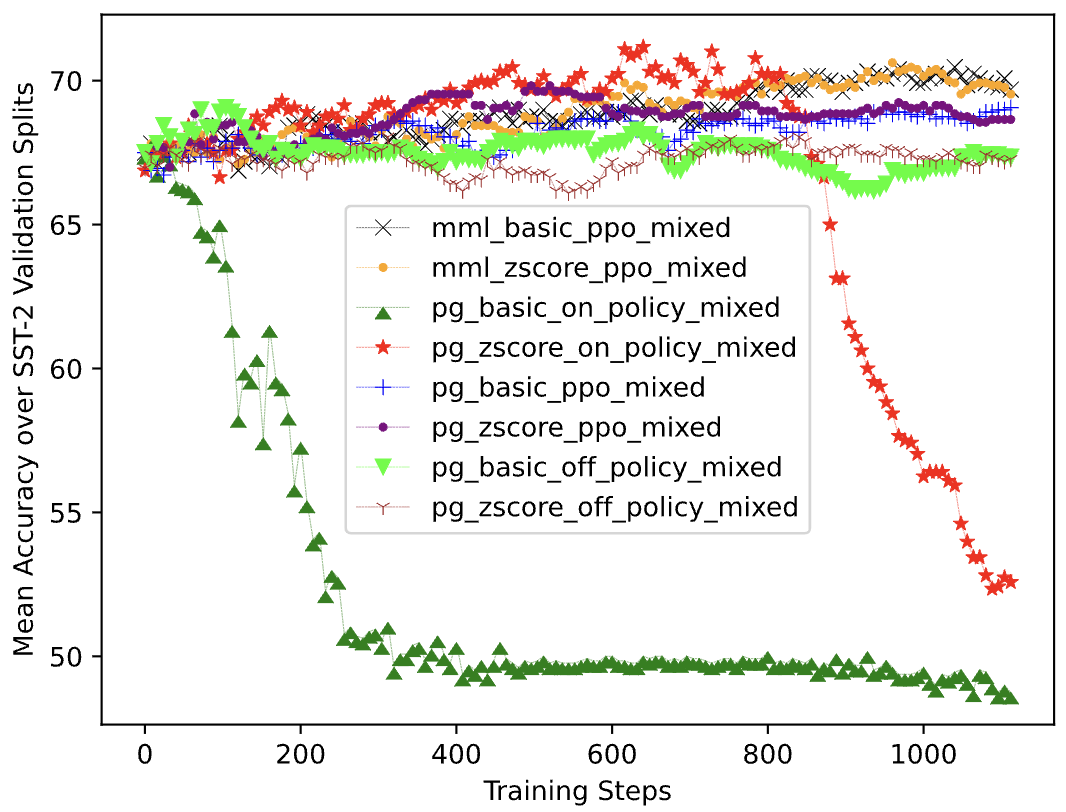
\includegraphics[width=0.45\textwidth]{mml_pg_comparisons.png}
\end{center}
\caption{Average ensemble accuracy over five validation splits in the 128-shot SST2 classification task. PG gradient estimation is not robust during the training trajectory while doing on-policy learning.}
\label{pg_divergence}
\end{figure}


We randomly select 128 training examples for each unique label within the dataset. An equal number of examples are gathered to form an internal validation set. We create five train/validation splits using the arbitrarily chosen random seeds \{11, 42, 1993, 12321, 2023\}. We train the models for 1120 training steps with the batch size of 8 (i.e. 35 epochs). As we are training the models, we evaluate the performance of 140 weight checkpoints per model on the validation splits (i.e one checkpoint per 8 training steps). We examine the mean accuracy, which is averaged over the five validation splits. Despite the ensembling approach described in Section~\ref{ensemble-inference}, to accurately capture the quality of the generated paraphrases, we exclude the original input $x$ when computing the ensemble accuracy on the validation splits.

We assess the impact of reward normalization in the context of on-policy, off-policy, and PPO learning, considering both PG and MML gradient estimations. Table~\ref{maximum-curves-on-ppo} lists the best performance out of all the checkpoints evaluated on the validation splits, which is further averaged over five validation splits. With both PG and MML gradient estimations, reward normalization is boosting the performance across the three text decoding techniques for both on-policy and PPO learning techniques (see `AVG' column in Table~\ref{maximum-curves-on-ppo}). Conversely, reward normalization is not improving performance with off-policy learning (follow discussion in Appendix~\ref{training-paraphrase-extra:appendix} and see Table~\ref{maximum-curves-off}).

Table~\ref{maximum-curves-on-ppo} verifies that MML gradient estimation outperforms PG gradient estimation on average across three decoding techniques for both on-policy and PPO learning techniques. The highest accuracy is acheived by `PG {\small + zscoring}' with on-policy learning and top-p decoding, however it is not robust during the entire training trajectory. Figure~\ref{pg_divergence} shows that PG gradient estimation is not robust throughout the training trajectory, which causes the paraphrase generator to produce nonsensical paraphrases.  This results in downstream classification performance on par with random guessing. In contrast, off-policy and PPO learning circumvent this divergence. MML gradient estimation maintains robustness throughout the training phase (further discussion in Table~\ref{average-curves-on-ppo} of Appendix~\ref{training-paraphrase-extra:appendix}).

Upon investigating various elements of our learning objectives for fine-tuning the paraphrase generator, the combination that delivers the best performance across the validation splits, which is also robust during the entire training trajectory, includes: MML gradient approximation, PPO learning, mixed decoding for sample generation, and finally applying reward normalization. We name this combined approach our proposed RIFF algorithm. Table~\ref{example-paraphrase} lists an example sentence with its generated paraphrases on the SST2 dataset. In the subsequent experiments, we applied RIFF to generate paraphrases that augment the training mini-batches while tuning the downstream language model in a few-shot setting.

\begin{comment}
For zero-shot prediction over the final evaluation splits, Table~\ref{RIFF-vs-main-zero-shot}
provides results of an ablation experiment investigating the effect of RIFF over our pre-trained paraphrase model. Appendix~\ref{training-paraphrase-examples:appendix} also provides some example paraphrases before and after fine-tuning the paraphrase model with RIFF.
\end{comment}



\subsection{Paraphrases for Few-shot LM Tuning}

\begin{table*}
\centering
\caption{Average accuracy on the standard evaluation sets for the 16-shot single-sentence text classification. The last column is the micro averaged performance across the datasets. Numbers in parentheses are the deltas compared to non-RIFF baseline per LM Tuning technique. Highest performance per dataset bolded, second highest underlined. $\dagger$: the average 16-shot fine-tuning results with automatically searched templates. $\star$: reported zero-shot results for GPT3 with in-context learning~\cite{gao-etal-2021-making}.}

\begin{tabular}{c | c | c | c | c | c | c | c || c }
\hline
Tuning Method & SST2 & SST5 & CR & MR & TREC & Subj & AGN & AVG \\
\small(LM = RoBERTa-large) &  &  &  &  &  &  &  & \\
\hline
\small GPT-3 | In-context Learning$\star$ & \small84.8 & \small30.6 & \small87.4 & \small80.5 & \small26.2 & \small 53.6 & \small - & \small64.4 \\
\small \cite{deng-etal-2022-rlprompt} (RLPrompt) & \small92.5 & \small41.4 & \small89.5 & \small\underline{87.1} & \small60.5 & \small81.9 & \small 80.2 & \small78.1 \\
\small \cite{gao-etal-2021-making}$\dagger$ & \small92.3 & \small49.2 & \small89.0 & \small85.5 & \small\underline{88.2} & \small\textbf{91.2} & \small - & \small80.9 \\
\hline
\small No Tuning + Instructions & \small84.6 & \small31.0 & \small77.8 & \small81.3 & \small27.6 & \small 57.7 & \small 51.5 & \small58.5 \\
\hline
\small +GS & \small85.5 & \small37.0 & \small80.2 & \small83.0 & \small45.3 & \small74.5 & \small 82.0 & \small74.9 \\
\tiny+RIFF (train) & \small86.4 & \small37.8 & \small82.7 & \small84.7 & \small51.0 & \small74.4 & \small 81.0 &\;\;\;\;\;\;\;\;\small75.3 (+0.4) \\
\tiny+RIFF (train+test) & \small87.3 & \small38.2 & \small85.1 & \small84.7 & \small52.4 & \small77.2 & \small 83.3 &\;\;\;\;\;\;\;\;\small77.0 (+2.1) \\
\hline
\small +SpTune & \small89.7 & \small39.4 & \small82.4 & \small86.1 & \small35.2 & \small72.4 & \small 82.0 & \small75.7 \\
\tiny+RIFF (train) & \small91.2 & \small44.5 & \small84.6 & \small86.1 & \small38.4 & \small79.7 & \small 84.0 &\;\;\;\;\;\;\;\;\small78.5 (+2.7) \\
\tiny+RIFF (train+test) & \small91.6 & \small45.1 & \small86.2 & \small86.6 & \small38.4 & \small81.6 & \small 86.0 &\;\;\;\;\;\;\;\;\small79.9 (+4.1) \\
\hline
\small +AllTune & \small93.1 & \small48.0 & \small89.2 & \small\textbf{87.3} & \small87.2 & \small85.8 & \small 87.7 & \small\underline{83.3}\\
\tiny+RIFF (train) & \small\underline{93.6} & \small\underline{50.6} & \small\underline{90.2} & \small85.8 & \small84.2 & \small85.3 & \small 87.2 &\;\;\;\;\;\;\;\;\small\underline{83.3} (+0.0)\\
\tiny+RIFF (train+test) & \small\textbf{93.8} & \small\textbf{51.2} & \small\textbf{91.0} & \small85.5 & \small84.4 & \small\underline{86.6} & \small 87.2 &\;\;\;\;\;\;\;\;\small\textbf{83.6} (+0.3)\\
\hline
\small +LoRA & \small92.5 & \small48.1 & \small88.6 & \small86.0 & \small\textbf{89.3} & \small81.5 & \small 87.3 & \small82.5 \\
\tiny+RIFF (train) & \small92.7 & \small48.0 & \small87.5 & \small85.1 & \small84.8 & \small81.9 & \small \underline{87.6} &\;\;\;\;\;\;\;\;\small82.3 (-0.2)\\
\tiny+RIFF (train+test) & \small93.1 & \small49.2 & \small89.0 & \small85.4 & \small85.9 & \small84.4 & \small \textbf{87.9} &\;\;\;\;\;\;\;\;\small83.1 (+0.6)\\
\hline
\end{tabular}
\label{RIFF-vs-main-16-shot}
\end{table*}

Our primary hypothesis is that various LM tuning techniques could benefit from diverse views of the original input text. To test this hypothesis, we fine-tuned our paraphrase generators in a 16-shot classification setup using the RIFF algorithm. Subsequently, we fine-tuned the downstream classification model in the same 16-shot setting, while introducing $M=8$ paraphrases as per the objective outlined in Equation~\ref{lmfp-augmentation-objective}. For evaluation, we used the best model from the validation set to make predictions on standard evaluation splits, following the ensemble approach described in Section~\ref{ensemble-inference}.
For consistency with prior research, we used the random dataset splits provided by RLPrompt~\cite{deng-etal-2022-rlprompt}, aligning with the random seeds used by LM-BFF~\cite{gao-etal-2021-making}.


Table~\ref{RIFF-vs-main-16-shot} illustrates the average accuracy on standard test sets across seven text classification datasets. The reported scores correspond to four distinct LM tuning techniques: GS, SpTune, AllTune, and LoRA. Results for ClsTune, HTune, and InTune are presented in Table~\ref{RIFF-vs-main-16-shot-rest} of Appendix~\ref{lm-tuning-extra:appendix}.

Notably, recent prompt optimization techniques (i.e. GS and SpTune) exhibit significant benefits from paraphrase augmentation during training. Particularly, SpTune demonstrates the most substantial improvement, with a 2.7\% increase in accuracy. Furthermore, LoRA consistently outperforms prompt optimization techniques, aligning with findings from prior studies~\cite{DBLP:journals/corr/abs-2106-09685}. Interestingly, paraphrase augmentation still aids LoRA in efficiently learning adaptation matrices, resulting in a 0.5\% accuracy increase on SST2, a 0.4\% accuracy boost on Subj, and a 0.3\% accuracy improvement on AGN datasets. Coupled with ensemble predictions, denoted in rows labeled `+RIFF (train+test)' all LM tuning techniques benefit from paraphrase augmentation.

\section{Related Works} % Alona stopped here Nov 21
To improve prompt optimization and efficient tuning techniques for LMs, we incorporate the generated paraphrases into the training mini-batches. It is important to note that data augmentation in NLP has been explored through various methods. Paraphrase generation represents just one technique of data augmentation. For a comprehensive overview of diverse data augmentation techniques for NLP tasks, we direct interested readers to a recent survey by \citet{DBLP:journals/corr/abs-2106-07499}.

\noindent
{\bf Prompt Optimization \& Efficient Tuning}: Recent research proposes various techniques for prompt optimization and efficient tuning of language models. In our experiments, we have used successful techniques from each of these areas. Appendix~\ref{related-works-extra:appendix} provides our detailed description of these recent techniques.
All of the recent techniques for prompt optimization and efficient tuning of the language models use the original input task (or the original input context) provided within the dataset.

\noindent
{\bf Paraphrase Generation}:
Our objective is not to present a state-of-the-art paraphrase generator, but rather to examine the impact of incorporating input paraphrases on the efficient tuning of LMs. Recent advancements in generating diverse paraphrases~\cite{zhou-bhat-2021-paraphrase} could provide better pre-trained models, thereby these techniques can enhance performance in all our experiments as our proposed RIFF technique can be seen as an extra fine-tuning step for the paraphrase model. These recent techniques encompass various approaches, including the use of copy mechanisms, Variational Autoencoders, Generative Adversarial Networks, and Reinforcement Learning techniques. For a comprehensive overview of neural paraphrase generation, please refer to a recent survey by Zhou and Bhat~\cite{zhou-bhat-2021-paraphrase}. While previous studies have applied RL techniques for paraphrase generation, we propose the use of MML gradients instead of policy gradients to fine-tune our paraphrase model.

\section{Conclusion}
We investigated the impact of incorporating input paraphrases while fine-tuning PLMs with recent prompt optimization and efficient tuning techniques. We also provided extensive experiments for reducing noise in a distantly supervised paraphrase generator.

Recent study suggests that large PLMs face constraints related to the quantity of unique data points~\cite{muennighoff2023scaling}. A potential avenue for future research could explore whether the introduction of paraphrased inputs can mitigate these challenges for large PLMs during the pre-training stage.

\section*{Limitations}
Our paraphrase generator is pre-trained on semi-supervised paraphrases given by a truly large language model (i.e. ChatGPT). Although these large models are capable of generating high quality paraphrases for the English language. It is not clear if these semi-supervised paraphrases are available for other languages.

Our investigation into the effects of paraphrases on efficient LM tuning techniques relies on language models that can be trained on commodity hardware. It would be interesting to explore how recent LLMs respond to input paraphrases. Nevertheless, it is important to note that tuning larger models, those with more than 30 billion parameters, requires access to the gradients, however, the gradients for proprietary models are not available.

Throughout this study, our primary focus has been on classification tasks. A potential avenue for future research could involve assessing the sensitivity of LM tuning techniques to input paraphrases in generative tasks.

To enhance language model tuning with paraphrases, we augment the training mini-batches. However, this approach does result in increased training time. It would be ideal to devise a form of regularization for efficient language model tuning, one that exposes the model's parameters to various paraphrases of the original input text.

\section*{Ethics Statement}
Many language models show biases in their output due to the data used to train them \cite{liang2021towards}.   It is possible that even with few-shot language model tuning, we might continue to detect analogous biases in the downstream classification task, for instance, resulting in diminished classification accuracy for specific minority groups.

\begin{comment}
\section*{Acknowledgements}
This document has been adapted by Jordan Boyd-Graber, Naoaki Okazaki, Anna Rogers from the style files used for earlier ACL, EMNLP and NAACL proceedings, including those for
EACL 2023 by Isabelle Augenstein and Andreas Vlachos,
EMNLP 2022 by Yue Zhang, Ryan Cotterell and Lea Frermann,
ACL 2020 by Steven Bethard, Ryan Cotterell and Rui Yan,
ACL 2019 by Douwe Kiela and Ivan Vuli\'{c},
NAACL 2019 by Stephanie Lukin and Alla Roskovskaya,
ACL 2018 by Shay Cohen, Kevin Gimpel, and Wei Lu,
NAACL 2018 by Margaret Mitchell and Stephanie Lukin,
Bib\TeX{} suggestions for (NA)ACL 2017/2018 from Jason Eisner,
ACL 2017 by Dan Gildea and Min-Yen Kan, NAACL 2017 by Margaret Mitchell,
ACL 2012 by Maggie Li and Michael White,
ACL 2010 by Jing-Shin Chang and Philipp Koehn,
ACL 2008 by Johanna D. Moore, Simone Teufel, James Allan, and Sadaoki Furui,
ACL 2005 by Hwee Tou Ng and Kemal Oflazer,
ACL 2002 by Eugene Charniak and Dekang Lin,
and earlier ACL and EACL formats written by several people, including
John Chen, Henry S. Thompson and Donald Walker.
Additional elements were taken from the formatting instructions of the \emph{International Joint Conference on Artificial Intelligence} and the \emph{Conference on Computer Vision and Pattern Recognition}.
\end{comment}

% Entries for the entire Anthology, followed by custom entries
\bibliography{my_bib}
\bibliographystyle{acl_natbib}

\appendix

\section{Few-shot Paraphrase Training (Further Results)}
\label{training-paraphrase-extra:appendix}


This section provides additional results that compare our training objectives for fine-tuning the paraphrase generator using the feedback from the downstream language model.

\begin{table}
\centering
\caption{The accuracy of the best performing validation checkpoints in the 128-shot SST2 classification task trained with the off-policy learning technique. Highest performance per column bolded. Last column reports the macro-average among each row.}
\begin{tabular}{c | c c c | c}
\hline
& \multicolumn{3}{c|}{Off-Policy} & AVG \\
Learn Tech & \small{Top-P} & \small{Beam} & \small{Mixed} & \\
\hline
No Tuning & \small67.5 & \small67.5 & \small67.5 & \small67.5 \\
\hline
PG & \small68.6 & \small68.4 & \small69.1 & \small68.7\\
PG \small +zscoring & \small68.8 & \small68.7 & \small68.0 & \small68.5 \\
\hline
MML & \small\textbf{69.2} & \small\textbf{70.1} & \small\textbf{70.1} & \small\textbf{69.8} \\
MML \small +zscoring & \small\textbf{69.2} & \small69.7 & \small\textbf{70.1} & \small69.7\\
\hline
\end{tabular}
\label{maximum-curves-off}
\end{table}

The off-policy learning technique improves performance when using basic rewards (i.e., 69.1\% compared to 67.9\% with mixed decoding). However, the combined effect of off-policy learning and reward normalization decreases performance. With mixed decoding, `PG {\small+ zscoring}' yields an accuracy of 71.2\% in on-policy learning compared to an accuracy of 68.0\% with off-policy learning. The `AVG' column in Table~\ref{maximum-curves-off} further verifies this conclusion that reward normalization is not improving the final performance while training the model with off-policy learning. We hypothesize that with the off-policy learning technique, the normalized rewards should be re-weighted properly if the sampled paraphrases are from the fixed paraphrase model.

\begin{table*}
\centering
\caption{The average accuracy computed over all the validation checkpoints in the 128-shot SST2 classification task. Highest performance per column bolded. Last column reports the macro-average among each row.}
\begin{tabular}{ c | c c c | c c c | c}
\hline

Learn Tech & \multicolumn{3}{c|}{On-Policy} & \multicolumn{3}{c|}{PPO} & AVG \\
 & \small{Top-P} & \small{Beam} & \small{Mixed} & \small{Top-P} & \small{Beam} & \small{Mixed} & \\
\hline
No Tuning \small + Instructions & \small67.5 & \small67.5 & \small67.5 & \small67.5 & \small67.5 & \small67.5 & \small67.5\\
\hline
+PG & \small 53.2 & \small 52.0 & \small 52.4 & \small 67.4 & \small 67.4 & \small 68.2 & \small 60.1 \\
+PG \small +zscoring & \small 63.8 & \small 68.6 & \small 66.6 & \small 67.6 & \small 67.9 & \small 68.5 & \small 67.2 \\
\hline
+MML& \small 68.5 & \small 67.6 & \small 68.6 & \small \textbf{68.2} & \small \textbf{69.0} & \small \textbf{68.9} & \small 68.5 \\
+MML \small +zscoring & \small \textbf{69.1} & \small \textbf{68.9} & \small \textbf{69.1} & \small 67.9 & \small \textbf{69.0} & \small \textbf{68.9} & \small \textbf{68.8} \\
\hline
\end{tabular}
\label{average-curves-on-ppo}
\end{table*}

In Table~\ref{average-curves-on-ppo}, we also report the average accuracy of all the checkpoints as we are training the models. The learning technique `MML {\small + zscoring}' is more robust during the training trajectory compared to `PG {\small + zscoring}'.


\begin{table*}
\centering
\caption{Generated paraphrases after fine-tuning the paraphrase model with the RIFF method for the following input sentence: ``It's difficult to get beyond the overall blandness of American chai, despite its likable performances and refreshingly naive point of view.''}

\begin{tabular}{ p{0.1\linewidth} | p{0.87\linewidth} }
\hline
Paraphrase & Text \\
\hline
P1 & ``Despite its enjoyable performances and refreshingly naive perspective, american chai is difficult to surpass due to its overall blandness.''\\
\hline
P2 & ``American chai's enjoyable performances and refreshing perspective make it difficult to elevate beyond its blandness.''\\
\hline
P3 & ``The overall blandness of American chai is difficult to overcome, despite its enjoyable performances and refreshingly naive perspective.''\\
\hline
P4 & `` It's difficult to surpass the blandness of American chai, even with its enjoyable performances and refreshingly naive perspective.
''\\
\hline
P5 & ``Although american chai has decent performances and a refreshingly naive viewpoint, it's difficult to elevate its overall blandness.
''\\
\hline
P6 & ``Americans chai is often bland, but it's difficult to surpass its enjoyable performances and refreshingly naive perspective.''\\
\hline
P7 & ``American Chai's lack of quality is difficult to overcome, even with enjoyable performances and a refreshing perspective.
''\\
\hline
P8 & ``Even with enjoyable performances and a refreshingly simplistic viewpoint, american chapin's blandness is difficult to shake off.''\\
\hline
\end{tabular}
\label{example-paraphrase}
\end{table*}



\begin{comment}
# skip, show if being asked by reviewers. Don't want to confuse the paper.
Finally, Table \ref{RIFF-vs-main-zero-shot} reports the effect of RIFF training for zero-shot prediction with the downstream language model in SST2 and SST5 datasets.

\end{comment}

\begin{comment}
# Skipping this table.
\begin{table}
\centering
\caption{Average accuracy on the standard evaluation sets for the SST2 (dev set) and SST5 (dev set) datasets in the zero-shot classification setting, where only RIFF trains the paraphrase generator in a $k$-shot setting. The language model is fixed. We also exclude the original evaluation set's input and rely on the ensemble performance of the generated paraphrases.}

\begin{tabular}{c | c | c | c }
\hline
 & SST2 & SST5 & AVG \\
Method &  &  & \\
\hline
\small - RIFF & \small72.3 & \small23.2 & \small47.8 \\
\small + RIFF (k=16) & \small73.0 & \small23.1 & \small48.1 \\
\small + RIFF (k=128) & \small\textbf{74.2} & \small\textbf{23.5} & \small\textbf{48.9} \\
\hline
\end{tabular}
\label{RIFF-vs-main-zero-shot}
\end{table}

\end{comment}

\section{Further Training Details}
\label{training-details-extra:appendix}

The learning rate for each LM tuning technique was separately fine-tuned from the set \{0.5, 0.3, 0.1, 0.01, 0.001, 0.0001, 0.00001\} using the train/validation split created for the seed 11 on the SST2 dataset. The tuned learning rates were then applied globally across other datasets and experiments. For paraphrase fine-tuning, we train all the parameters in T5-base with the learning rate of 0.00001. In Tables~\ref{hyper-parameters} and~\ref{learning-rates}, we list the hyper-parameters and learning rates used across all datasets.  For optimization, we utilized the AdamW~\cite{DBLP:journals/corr/abs-1711-05101}\footnote{\url{https://pytorch.org/docs/stable/generated/torch.optim.AdamW.html}} optimizer with the AMSGrad variant set to True~\cite{DBLP:journals/corr/abs-1904-09237}. We implemented the methods using the HuggingFace\footnote{\url{https://huggingface.co/}} library and the PyTorch\footnote{\url{https://pytorch.org/}} machine learning framework. We report the accuracy metric on these classification datasets. The experiments were conducted using multiple NVIDIA's A40 GPU cards.
% This was facilitated by the GPU cluster provided by the Vector Institute\footnote{\url{https://vectorinstitute.ai/}}.

\begin{table}[t]
\centering
\caption{Shared hyper-parameters used across all experiments and datasets.}
\begin{tabular}{ c | c }
\hline
Hyper-parameter & Value\\
\hline
Top-$k$ candidates in GS & $k$=4 \\
batch size (RoBERTa-large) & 8 \\
batch size in GS (RoBERTa-large) & 2 \\
%batch size (T5-3B) & 2 \\
Weight decay & 0.0001 \\
Max epochs & 100 \\
length cutoff & 128 tokens \\
Paraphrase sample size & $M$=8 \\
Checkpointing steps & 8 \\
$D^{'}$ in ClsTune & 128 \\
Prompt len in SpTune & $L$=25 \\
$\beta$ in MML & 0.1 \\
$\beta$ in PG & 0.6 \\
Lora $\alpha$ & 32 \\
Lora $r$ & 8 \\
Lora dropout & 0.1 \\
Diversity penalty for Div beam & 3.0 \\
Repetition penalty for Div beam & 10.0 \\
Temperature in Div beam & 0.7 \\
P value for top-p & 0.99
\end{tabular}
\label{hyper-parameters}
\end{table}

\begin{table}[t]
\centering
\caption{Learning rates used per Language Model (LM) tuning technique.}
\begin{tabular}{ c | c }
\hline
LM Tuning Technique & Learning Rate\\
\hline
GS & No rate \\
%GrIPS & No rate \\
AllTune & 0.00001 \\
InTune &  0.001 \\
HTune & 0.001 \\
ClsTune & 0.001 \\
SpTune & 0.001 \\
LoRA & 0.0001
\end{tabular}
\label{learning-rates}
\end{table}


\section{Paraphrases for Few-shot LM Tuning (Further Results)}
\label{lm-tuning-extra:appendix}
Due to space limitations, we present the results for ClsTune, HTune, and InTune in Table~\ref{RIFF-vs-main-16-shot-rest}.
\begin{table*}
\centering
\caption{Average accuracy on the standard evaluation sets for the 16-shot single-sentence text classification using the ClsTune, HTune, and InTune fine-tuning techniques. The last column is the micro averaged performance across the datasets.}

\begin{tabular}{c | c | c | c | c | c | c | c || c }
\hline
Tuning Method & SST2 & SST5 & CR & MR & TREC & Subj & AGN & AVG \\
\small(LM = RoBERTa-large) &  &  &  &  &  &  &  & \\
\hline
\small ClsTune & \small72.6 & \small34.4 & \small71.4 & \small67.3 & \small74.8 & \small87.7 & \small 81.7 & \small72.8 \\
\tiny+RIFF (train)  & \small72.5 & \small33.9 & \small68.3 & \small70.3 & \small75.8 & \small88.4 & \small 84.0 &\;\;\;\;\;\;\;\;\small73.8 (+1.0) \\
\tiny+RIFF (train+test)  & \small74.0 & \small35.0 & \small71.1 & \small72.0 & \small76.8 &\small 89.4 & \small 84.9 &\;\;\;\;\;\;\;\;\small75.1 (+2.3)\\
\hline
\small HTune & \small87.4 & \small37.4 & \small84.0 & \small83.1 & \small62.4 & \small83.8 & \small 81.4 & \small76.9 \\
\tiny+RIFF (train) & \small88.1 & \small40.3 & \small84.5 & \small83.4 & \small70.7 & \small87.3 & \small 83.4 &\;\;\;\;\;\;\;\;\small78.8 (+2.0) \\
\tiny+RIFF (train+test) & \small89.1 & \small40.4 & \small86.4 & \small83.2 & \small71.6 & \small87.8 & \small 85.2 &\;\;\;\;\;\;\;\;\small80.0 (+3.1) \\
\hline
\small InTune & \small91.5 & \small42.3 & \small87.3 & \small84.0 & \small67.7 & \small82.7 & \small 83.8 & \small79.4 \\
\tiny+RIFF (train) & \small92.6 & \small43.2 & \small87.5 & \small85.9 & \small63.8 & \small82.7 & \small 85.6 &\;\;\;\;\;\;\;\;\small80.5 (+1.1) \\
\tiny+RIFF (train+test) & \small93.1 & \small43.9 & \small89.0 & \small85.9 & \small69.6 & \small84.6 & \small 86.9 &\;\;\;\;\;\;\;\;\small81.7 (+2.3)\\
\hline
\end{tabular}
\label{RIFF-vs-main-16-shot-rest}
\end{table*}

\begin{table*}
\centering
\caption{Average accuracy on the standard evaluation sets for the 16-shot single-sentence text classification. The last column is the micro averaged performance across the datasets. Numbers in parentheses are the deltas compared to non-RIFF baseline per LM Tuning technique.}

\begin{tabular}{c | c | c | c | c | c | c | c || c }
\hline
Tuning Method & SST2 & SST5 & CR & MR & TREC & Subj & AGN & AVG \\
\hline
\small (LM = T5-large) &  &  &  &  &  &  &  & \\
\small No Tuning + Instructions & \small49.9 & \small23.1 & \small50.0 & \small50.0 & \small18.8 & \small 50.8 & \small 13.4 & \small0.0 \\
    \small +LoRA & \small92.0 & \small47.6 & \small91.9 & \small84.5 & \small86.9 & \small87.0 & \small86.1 & \small0.0 \\
\tiny+RIFF (train) & \small91.7 & \small46.6 & \small92.0 & \small85.7 & \small0.0 & \small86.0 & \small 0.0 &\;\;\;\;\;\;\;\;\small0.0 (-0.0)\\
\tiny+RIFF (train+test) & \small91.5 & \small47.1 & \small92.1 & \small85.4 & \small0.0 & \small86.7 & \small 0.0 &\;\;\;\;\;\;\;\;\small0.0 (+0.0)\\
\hline
\end{tabular}
\label{RIFF-vs-lora-other-lms}
\end{table*}

\section{Extended Related Works}
\label{related-works-extra:appendix}

\noindent
{\bf Prompt Optimization \& Efficient Tuning}: Recent research proposes various techniques for prompt optimization and efficient tuning of language models. In our experiments, we have used successful techniques from each of these areas.

FluentPrompt~\cite{shi2022human} is a recent discrete prompting technique based on the projected gradient-descent and Langevin dynamics. FluentPrompt introduces a fluency constraint within Langevin dynamics to generate a sample of high-performing prompts for more interpretable analysis of these discrete prompts. The optimized prompts by FluentPrompt performs on-par to the AutoPrompt, however they have lower perplexity~\cite{shi2022human}.

Building upon SpTune~\cite{lester-etal-2021-power} and P-tuning~\cite{li-liang-2021-prefix}, P-tuning V2~\cite{liu-etal-2022-p} introduced the concept of deep prompt tuning. This method involves injecting prompt vectors into the deeper layers of the transformer model to close the performance gap with AllTuning in medium-sized language models. We have experimented with LoRA~\cite{DBLP:journals/corr/abs-2106-09685}, a recent low-rank adaptation technique for tuning language models. Other potential methods include training bottleneck adapter modules~\cite{DBLP:journals/corr/abs-1902-00751, lin-etal-2020-exploring} added per sub-layer of the transformer model. LoRA outperforms adapter tuning and P-Tuning V2 techniques ~\cite{DBLP:journals/corr/abs-2106-09685}. The successors of LoRA include DyLoRA~\cite{valipour-etal-2023-dylora}  which dynamically learns a range of adaptation ranks, thus eliminating the need to search the rank of the adaptation matrices as a hyper-parameter. Similarly, AdaLoRA dynamically allocates the parameter budget among the weight matrices during adaptation, with matrices of higher priority (i.e., those with greater importance to the downstream task) receiving higher adaptation ranks than less important matrices~\cite{zhang2023adaptive}.

In scenarios where gradients are absent, Black-Box Tuning~\cite{DBLP:journals/corr/abs-2201-03514} applies derivative-free algorithms for optimizing continuous prompts. For discrete prompt optimization, RLPrompt~\cite{deng-etal-2022-rlprompt} employs the on-policy version of soft Q-learning~\cite{https://doi.org/10.48550/arxiv.2106.07704} to find the optimal prompt tokens in a gradient-free setting. Decoder Tuning~\cite{cui-etal-2023-decoder} learns a decoder network over the language model, thus circumventing the need for gradient computation and input-side prompt tuning in few-shot classification. In a recent study, TEMPERA~\cite{zhang2022tempera} introduced a novel approach that involves test-time discrete prompt editing using a trained RL agent. This agent is capable of modifying the instruction, in-context examples, or the verbalizers based on the given task input.

The use of Language Models (LLMs) in generating instructions for downstream tasks has involved a two-step process. Initially, LLMs generate a set of candidate instructions, and subsequently, the highest-scoring instruction is utilized to prompt another LLM to perform the downstream task. This approach, known as prompt-based generation-then-filtering, has been investigated in the recent APE method~\cite{zhou2023large}. APE demonstrates the ability to generate prompts that achieve performance comparable to human-designed prompts~\cite{zhou2023large}.

To prompt language models for reasoning tasks, another line of research augment the input context with demonstration examples outlining the intermediate reasoning steps to form the answer. Providing manually or automatically generated chain-of-thoughts within these demonstrations strikingly improve LLMs performance in reasoning tasks~\cite{DBLP:journals/corr/abs-2201-11903, zhang2022automatic, NEURIPS2022_8bb0d291}.

All of the aforementioned techniques for prompt optimization and efficient tuning of the language model use the original task's input text (or the original input context) provided within the dataset.

\noindent
{\bf RL for Paraphrase Generation}:
In the following paragraphs, we provide a brief overview of similar reinforcement learning objectives employed for paraphrase generation. Li et al.~\cite{li-etal-2018-paraphrase} used a deep RL technique, training a pointer-generator network as the paraphrase generator and a decomposable attention model as the evaluator which assigns a paraphrase score to pairs of sentences. The generator was trained using the policy gradient objective, with reward shaping and scaling to stabilize the training process~\cite{li-etal-2018-paraphrase}. Another approach by Qian et al.~\cite{qian-etal-2019-exploring} focused on generating diverse paraphrases by training multiple generators, accompanied by a paraphrase discriminator and a generator discriminator. Policy gradient objective and self-critical learning~\cite{DBLP:journals/corr/RennieMMRG16} were employed for training the generators, with the baseline reward used in the policy gradient objective being the reward obtained from the greedy-decoded sequence. Liu et al.~\cite{liu-etal-2020-learning} also applied the policy gradient objective with self-critical learning, incorporating multiple reward functions such as Rouge score with the reference paraphrase, negative Rouge score with the input sentence to encourage lexical variations, and semantic similarity score between the paraphrase and the input sentence to ensure semantic fidelity.

Another study by Du and Ji~\cite{du-ji-2019-empirical} compared the use of imitation learning algorithm DAGGER with policy gradient REINFORCE for paraphrase generation. The policy gradient objective has also been applied in generating paraphrases while considering multiple objectives for entailment relation-aware paraphrase generation~\cite{Sancheti_Srinivasan_Rudinger_2022}. In the context of chatbot responses, a recent work studies unsupervised paraphrase generation with proximal policy optimization, aiming to maximize a combination of rewards such as textual entailment, semantic similarity, language fluency, and lexical dissimilarity~\cite{DBLP:journals/corr/abs-2103-12777}. Similarly, the policy gradient objective has been employed to optimize multiple rewards, similar to previous work, for unsupervised paraphrase generation~\cite{10.1145/3394486.3403231}.

While previous studies have applied RL techniques for paraphrase generation, we propose the use of MML gradients instead of policy gradients to train our paraphrase model.

\section{Task Instructions \& Input Format}
\label{task-instruct-input-format:appendix}
Table~\ref{task-input-format} provides a summary of the task instructions that we append before the inputs, as well as the class verbalizers for classifying the input text. The instructions and input templates are derived from prior work in prompt optimization~\cite{deng-etal-2022-rlprompt}.

%For T5-3B model, we remove the prefix `<s>', and replace the token `<mask>' with the token `<extra\_id\_0>' to be consistent with the T5's pre-training format.

\begin{table*}
\centering
\caption{Number of classes $C$, the input format, and the instruction used per dataset. The label words are provided within the instructions.}
\begin{tabular}{ p{0.1\linewidth} | p{0.05\linewidth} | p{0.2\linewidth} | p{0.5\linewidth} }
\hline
Dataset & $C$ & Input Format & Instruction \\
\hline
SST2 & 2 & ``<s> \{Instruction\} \{Text\} . It was <mask> . </s>'' & ``In this task, you are given sentences from movie reviews. The task is to classify a sentence as `great' if
the sentiment of the sentence is positive or as `terrible' if the sentiment of the sentence is negative.''\\
\hline
SST5 & 5 & ``<s> \{Instruction\} \{Text\} . It was <mask> . </s>'' & ``In this task, you are given sentences from movie reviews. Based on the given review, classify it to one of
the five classes: (1) terrible, (2) bad, (3) okay, (4) good, and (5) great.''\\
\hline
CR & 2 & ``<s> \{Instruction\} \{Text\} . It was <mask> . </s>'' & ``In this task, you are given sentences from customer reviews. The task is to classify a sentence as `great' if
the sentiment of the sentence is positive or as `terrible' if the sentiment of the sentence is negative.''\\
\hline
MR & 2 & ``<s> \{Instruction\} \{Text\} . It was <mask> . </s>'' & ``In this task, you are given sentences from movie reviews. The task is to classify a sentence as `great' if
the sentiment of the sentence is positive or as `terrible' if the sentiment of the sentence is negative.''\\
\hline
TREC & 6 & ``<s> \{Instruction\} <mask>: \{Text\} . </s>'' & ``You are given a question. You need to detect which category better describes the question. Answer with `Description', `Entity', `Expression', `Human', `Location', and `Number'.'' \\
\hline
Subj & 2 & ``<s> \{Instruction\} \{Text\} . This is <mask> . </s>'' & ``In this task, you are given sentences from reviews. The task is to classify a sentence as `subjective' if the
opinion of the sentence is subjective or as `objective' if the opinion of the sentence is objective.''\\
\hline
AG's News & 4 & ``<s> \{Instruction\} <mask> News: \{Text\} . </s>'' & ``In this task, you are given a news article. Your task is to classify the article to one out of the four topics
`World', `Sports', `Business', `Tech' if the article's main topic is relevant to the world, sports, business,
and technology, correspondingly. If you are not sure about the topic, choose the closest option.''\\
\hline
\end{tabular}
\label{task-input-format}
\end{table*}

\end{document}
